\documentclass{beamer}
\usepackage{color}
\usepackage{graphicx}
\usepackage{tikz}
\usepackage{listings}
\usepackage{tikz-qtree}
\usepackage[backend=bibtex]{biblatex}

\usetikzlibrary{arrows,positioning,decorations.pathreplacing,fit}

\usetheme{fibeamer}

\newcommand{\hl}{\textcolor{fibeamer@darkColor1}}

\newif\ifstartedinmathmode
\newcommand{\animcb}[4]{%
\begingroup%
\relax\ifmmode\startedinmathmodetrue\else\startedinmathmodefalse\fi%
\setlength{\fboxsep}{1pt}%
\only<#1>{\vphantom{gbf}#4}\only<#2>{\colorbox{#3}{\vphantom{gbf}\ifstartedinmathmode$#4$\else#4\fi}}%
\endgroup}

\newcommand{\pred}[1]{\animcb{1}{2-}{fibeamer@lightColor1}{#1}}
\newcommand{\func}[1]{\animcb{1}{2-}{fibeamer@lightColor2}{#1}}
\newcommand{\quant}[1]{\animcb{1}{2-}{fibeamer@lightColor3}{#1}}

%% ===   DEFINITIONS   ===

\tikzstyle{tex1} = [minimum width=3cm, minimum height=1cm, text centered]
\tikzstyle{tef1} = [minimum width=2.4cm, minimum height=1cm, text centered]
\tikzstyle{tsml} = [minimum width=3cm, text centered, font=\footnotesize]
\tikzstyle{box1} = [rectangle, rounded corners, minimum width=3cm,
                    minimum height=1cm, text centered, draw=fibeamer@color1,
                    fill=fibeamer@lightColor1]
\tikzstyle{box2} = [rectangle, rounded corners, minimum width=3cm,
                    minimum height=1cm, text centered, draw=fibeamer@color2,
                    fill=fibeamer@lightColor2]

\tikzset{
    invisible/.style={opacity=0},
    visible on/.style={alt={#1{}{invisible}}},
    alt/.code args={<#1>#2#3}{%
        \alt<#1>{\pgfkeysalso{#2}}{\pgfkeysalso{#3}} % \pgfkeysalso doesn't change the path
    }
}

\lstdefinestyle{imp}{
	morekeywords={TEST,THEN,ELSE,FI,WHILE,DO,END,SKIP,true,false,:=},
  keywordstyle=\bfseries,
  moredelim=**[is][\color{fibeamer@darkColor1}]{@}{@},
}

\lstdefinestyle{synquid}{
	morekeywords={List,Nat,Int,Bool},
	keywordstyle=\color{fibeamer@color1},
	classoffset=1,
	morekeywords={len},
	keywordstyle=\color{fibeamer@color2}
}

\bibliography{references.bib}

%% === END DEFINITIONS ===

\title{Program Synthesis}
\subtitle{An overview of logic-based approaches}
\author{Ricardo Brancas}
\institute{Instituto Superior Técnico}

\AtBeginSection[]{
\begin{frame}
    \frametitle{Presentation Outline}
    \tableofcontents[currentsection]
\end{frame}
}

\begin{document}

\begin{frame}
    \titlepage
\end{frame}

\section{What is it?}

\begin{frame}
    \frametitle{Program Synthesis}

    \centering
    \begin{tikzpicture}[node distance=2cm]

        \node[box1] (spec)                     {Specification};
      \onslide<2->{
        \node[box1] (synth) [below of = spec]  {Synthesiser};
      }
        \node[box1] (prog)  [below of = synth] {Program};

      \onslide<2->{
        \node[tsml] (spec1) [right = .75cm of spec, align=left] {Input/Output Examples\\
                                                                 First-order Logic Specification\\
                                                                 Hoare Logic Specification\\
                                                                 Separation Logic Specification\\
                                                                 ...};
        \draw[decorate,decoration={brace, raise=7pt, amplitude=5pt}] (spec1.south west) -- (spec1.north west);
      }

      \onslide<2->{
        \draw[->] (spec)  -- (synth);
        \draw[->] (synth) -- (prog);
      }

    \end{tikzpicture}
\end{frame}

\begin{frame}
    \frametitle{Formal Verification}

    How can we check if a program is correct (wrt. the specification)?\\~\\
    \pause
    We can use a logic formulation.

\end{frame}

\section{Logic Background}


\begin{frame}
    \frametitle{First-order Logic I}

    \begin{block}{First-order Logic (FOL)}
        A superset of \hl{propositional logic}, adding \animcb{1-1}{2-}{fibeamer@lightColor1}{predicates},
				\animcb{1-1}{2-}{fibeamer@lightColor2}{functions} and \animcb{1-1}{2-}{fibeamer@lightColor3}{quantifiers}.
    \end{block}

		\only<1>{
			\begin{exampleblock}{Propositional Logic}
	        $P \wedge Q$\\
	        $Q \implies P \vee R$\\
	    \end{exampleblock}
		}

		\mathchardef\mhyphen="2D

		\only<2->{
			\begin{exampleblock}{First-order Logic}
				$\quant{\forall} x. \pred{Panda}(x) \implies \pred{Mammal}(x)$\\
				$\neg \quant{\exists} x. \pred{Panda}(x) \wedge \neg\pred{Panda}(\func{father\mhyphen of}(x))$\\
	    	\end{exampleblock}
		}
\end{frame}

\begin{frame}
    \frametitle{First-order Logic II}

		\begin{block}{Validity \& Satisfiability}
	    	A formula is \hl{satisfiable} if it is True for some assignment to the variables/functions.\\
				It is \hl{valid} if it is True for all possible assignments.
		\end{block}

		\pause

		\begin{alertblock}{FOL Decidability}
				First-order logic is undecidable.
		\end{alertblock}

\end{frame}

\begin{frame}
    \frametitle{Decidability}

    \begin{block}{Decidable Problem}
        A problem is \hl{decidable} iff there is a way of deriving the correct answer.
    \end{block}

		\begin{block}{Undecidable Problem}
        Complementary, if a problem is \hl{undecidable} then it is \textit{provably
				impossible} to create an algorithm that always derives the correct answer.
    \end{block}~\\

		\pause
		As such, it is impossible to determine if any given formula is valid.\\
		So how can we solve this?

\end{frame}

\begin{frame}
    \frametitle{Satisfiability Modulo Theories}

    \begin{block}{Satisfiability Modulo Theory (SMT)}
		A decision problem on \hl{decidable subsets} of first-order logic.\\
		Such subsets are called \hl{theories}.
    \end{block}

		\begin{exampleblock}{Theory: Presburger arithmetic - $\{I\!N, +\}$}
        $3x + 2y < 3$\\
        $x + y + z = 45$
    \end{exampleblock}

		\pause

		\begin{exampleblock}{Theory: Equality with Uninterpreted Functions}
        $f(b) = d \; \wedge \; f(a) = d \; \wedge \; a = d$
    \end{exampleblock}

\end{frame}

\begin{frame}
    \frametitle{Satisfiability Modulo Theories - Models}

    % \begin{block}{$T$-satisfiability}
    %     Given a theory \hl{$T$}, we say that a formula \hl{$\Phi$} is \hl{$T$}-satisfiable iff there is some model \hl{$M$} of \hl{$T$}, such that \hl{$\Phi$} holds in \hl{$M$}.
    % \end{block}
    A model can be seen as a mapping from variables to constants/functions, and represents
		a solution of the formula.\\~\\

		\begin{exampleblock}{Example: Model for $\{3x + 2y < 3\}$}
				$\{ x \mapsto 0, y \mapsto 1\}$
		\end{exampleblock}

		\pause

		\begin{exampleblock}{Example: Model for $\{f(b) = d \; \wedge \; f(a) = d \; \wedge \; a = d\}$}
				$\{ a \mapsto *_1,\; b \mapsto *_2,\; d \mapsto *_1,\; f \mapsto \lambda x. *_1\}$
		\end{exampleblock}
\end{frame}

\begin{frame}
    \frametitle{Other Useful Theories for PL}

    \begin{itemize}
        \item Bit vectors
        \item Arrays
        \item Pointer logic
        \item Quantified Theories
				\item ...
    \end{itemize}~\\

		Different theories can also be combined while retaining decidability.
\end{frame}

\begin{frame}[fragile]
    \frametitle{Formal Verification}

    How can we check if a program is correct (wrt. to the specification)?\\
    We can use a logic formulation.\\

    \begin{columns}[T] % align columns
        \begin{column}{.48\textwidth}
            \begin{exampleblock}{Simple Hoare Triple}
                \vspace*{-.2\baselineskip}
				\begin{lstlisting}[xleftmargin=1em, escapechar=!,style=imp]
!\animcb{1-1}{2-}{fibeamer@lightColor1}{\{ X = 3 \}}!
Y ::= X - 2;;
X ::= X - 1
!\animcb{1-1}{2-}{fibeamer@lightColor2}{\{ X = 2 $\wedge$ Y = 1\}}!

                \end{lstlisting}
            \end{exampleblock}
        \end{column}\pause%
        \begin{column}{.48\textwidth}
            \begin{exampleblock}{SMT Formula}
                \vspace*{-1.5\baselineskip}
                \begin{align*}\footnotesize& \tikz[baseline]{\node[fill=fibeamer@lightColor1,anchor=base] (t2) {$X_0 = 3$};} \\
                    \wedge \enspace & Y_0 = (X_0 - 2) \\
                    \wedge \enspace & X_1 = (X_0 - 1) \\
                    \wedge \enspace & \tikz[baseline]{\node[fill=fibeamer@lightColor2,anchor=base] (t2) {$X_1 = 2 \wedge Y_0 = 1$};}
                \end{align*}
                \vspace*{-1\baselineskip}
            \end{exampleblock}
        \end{column}%
    \end{columns}~\\
    \pause
    We say that a program is correct, if the corresponding SMT formula is satisfiable.
\end{frame}

\section{A very simple synthesiser}

\begin{frame}
    \frametitle{Generating Programs}

    Now we can check if a given program is correct. But how do we generate them?\\~\\

    \pause

    \begin{block}{Enumeration}
        We can use the grammar of the language to generate (enumerate) all possible programs.
    \end{block}

    \pause

    \begin{alertblock}{Problem}
        The space of possible programs of fixed length, is exponentially large. It is impossible to just check all programs.
    \end{alertblock}
\end{frame}

\begin{frame}
    \frametitle{Generating Programs (Imp language)}

    \resizebox{\textwidth}{!}{%
        \begin{tikzpicture}
            \tikzset{level distance=90pt}
            \Tree
                [. \node {$\hl{com}$};
                    [. \node {$CSkip$};]
                    [. \node {$CAss(\hl{x}, \hl{aexp})$};
                        [. \node {$CAss(``a", \hl{aexp})$};
                            [. \node {$CAss(``a", ANum(\hl{n}))$};
                                [. \node {...}; ]
                            ]
                            [. \node {$CAss(``a", APlus(\hl{aexp_1}, \hl{aexp_2}))$};
                                [. \node {...}; ]
                            ]
                            [. \node {...};]
                        ]
                        [. \node {$CAss(``b", \hl{aexp})$};
                            [. \node {...}; ]
                        ]
                        [. \node {...};]
                    ]
                    [.\node {$CSeq(\hl{com_1}, \hl{com_2})$};
                        [. \node {...}; ]
                    ]
                    [.\node {$CIf(\hl{bexp}, \hl{com_1}, \hl{com_2})$};
                        [. \node {...}; ]
                    ]
                    [.\node {$CWhile(\hl{bexp}, \hl{com})$};
                        [. \node {...}; ]
                    ]
                ];
        \end{tikzpicture}
    }

\end{frame}

% \begin{frame}[fragile]
%     \frametitle{(Simple) Deduction Engine}
%
% 	The job of the deduction engine is:
%
% 	\begin{itemize}
% 		\item To prune the search when incorrect programs are generated.
% 	\end{itemize}
%
% % 	\begin{exampleblock}{Example}
% % 		\begin{lstlisting}[style=imp]
% % @TODO@
% % 		\end{lstlisting}
% % 	\end{exampleblock}
%
% \end{frame}

\begin{frame}
    \frametitle{The simplest synthesiser}

	\centering
    \begin{tikzpicture}[node distance=2cm]

        \node[box1] (enum) [] {Enumerator};
        \node[box1] (dedu) [below of = enum] {Program Checker};

		\node[draw,dotted,fit=(enum) (dedu)] (synt) {};

		\node[tef1] (spec) [left  = .5cm of synt] {Specification};
		\node[tef1] (prog) [right = .5cm of synt] {Program};

		\draw[->]   (spec)  -- (synt.west);
		\draw[->]   (synt.east) -- (prog);

		\draw[->]   ([xshift=1em]enum.south) -- ([xshift=1em]dedu.north);
		\draw[->]   ([xshift=-1em]dedu.north) -- ([xshift=-1em]enum.south);

    \end{tikzpicture}~\\~\\

	\pause

	\begin{alertblock}{Problem}
		This idea is very simple, but it has a big problem: most of the time is spent
		testing very similar programs that will never lead to a solution.
	\end{alertblock}

\end{frame}

\begin{frame}
	\frametitle{Possible Improvements}

	\begin{itemize}
		\item Domain Specific Languages (DSL)
		\item Partial evaluation
		\item Conflict-driven learning
		\item Type theory
		\item Synthetic separation logic
		\item ...
	\end{itemize}

\end{frame}

\section{A modern synthesiser: Synquid}

\begin{frame}
	\frametitle{\textbf{Synquid} \cite{polikarpova_program_2016}}

	\begin{columns}[c] % align columns
		\begin{column}{.48\textwidth}
			Synquid is a modern synthesiser that uses \textit{polymorphic refinement types}
			in order to prune the search space and make deductions about the program.
		\end{column}%
		\begin{column}{.48\textwidth}%
			\begin{figure}
				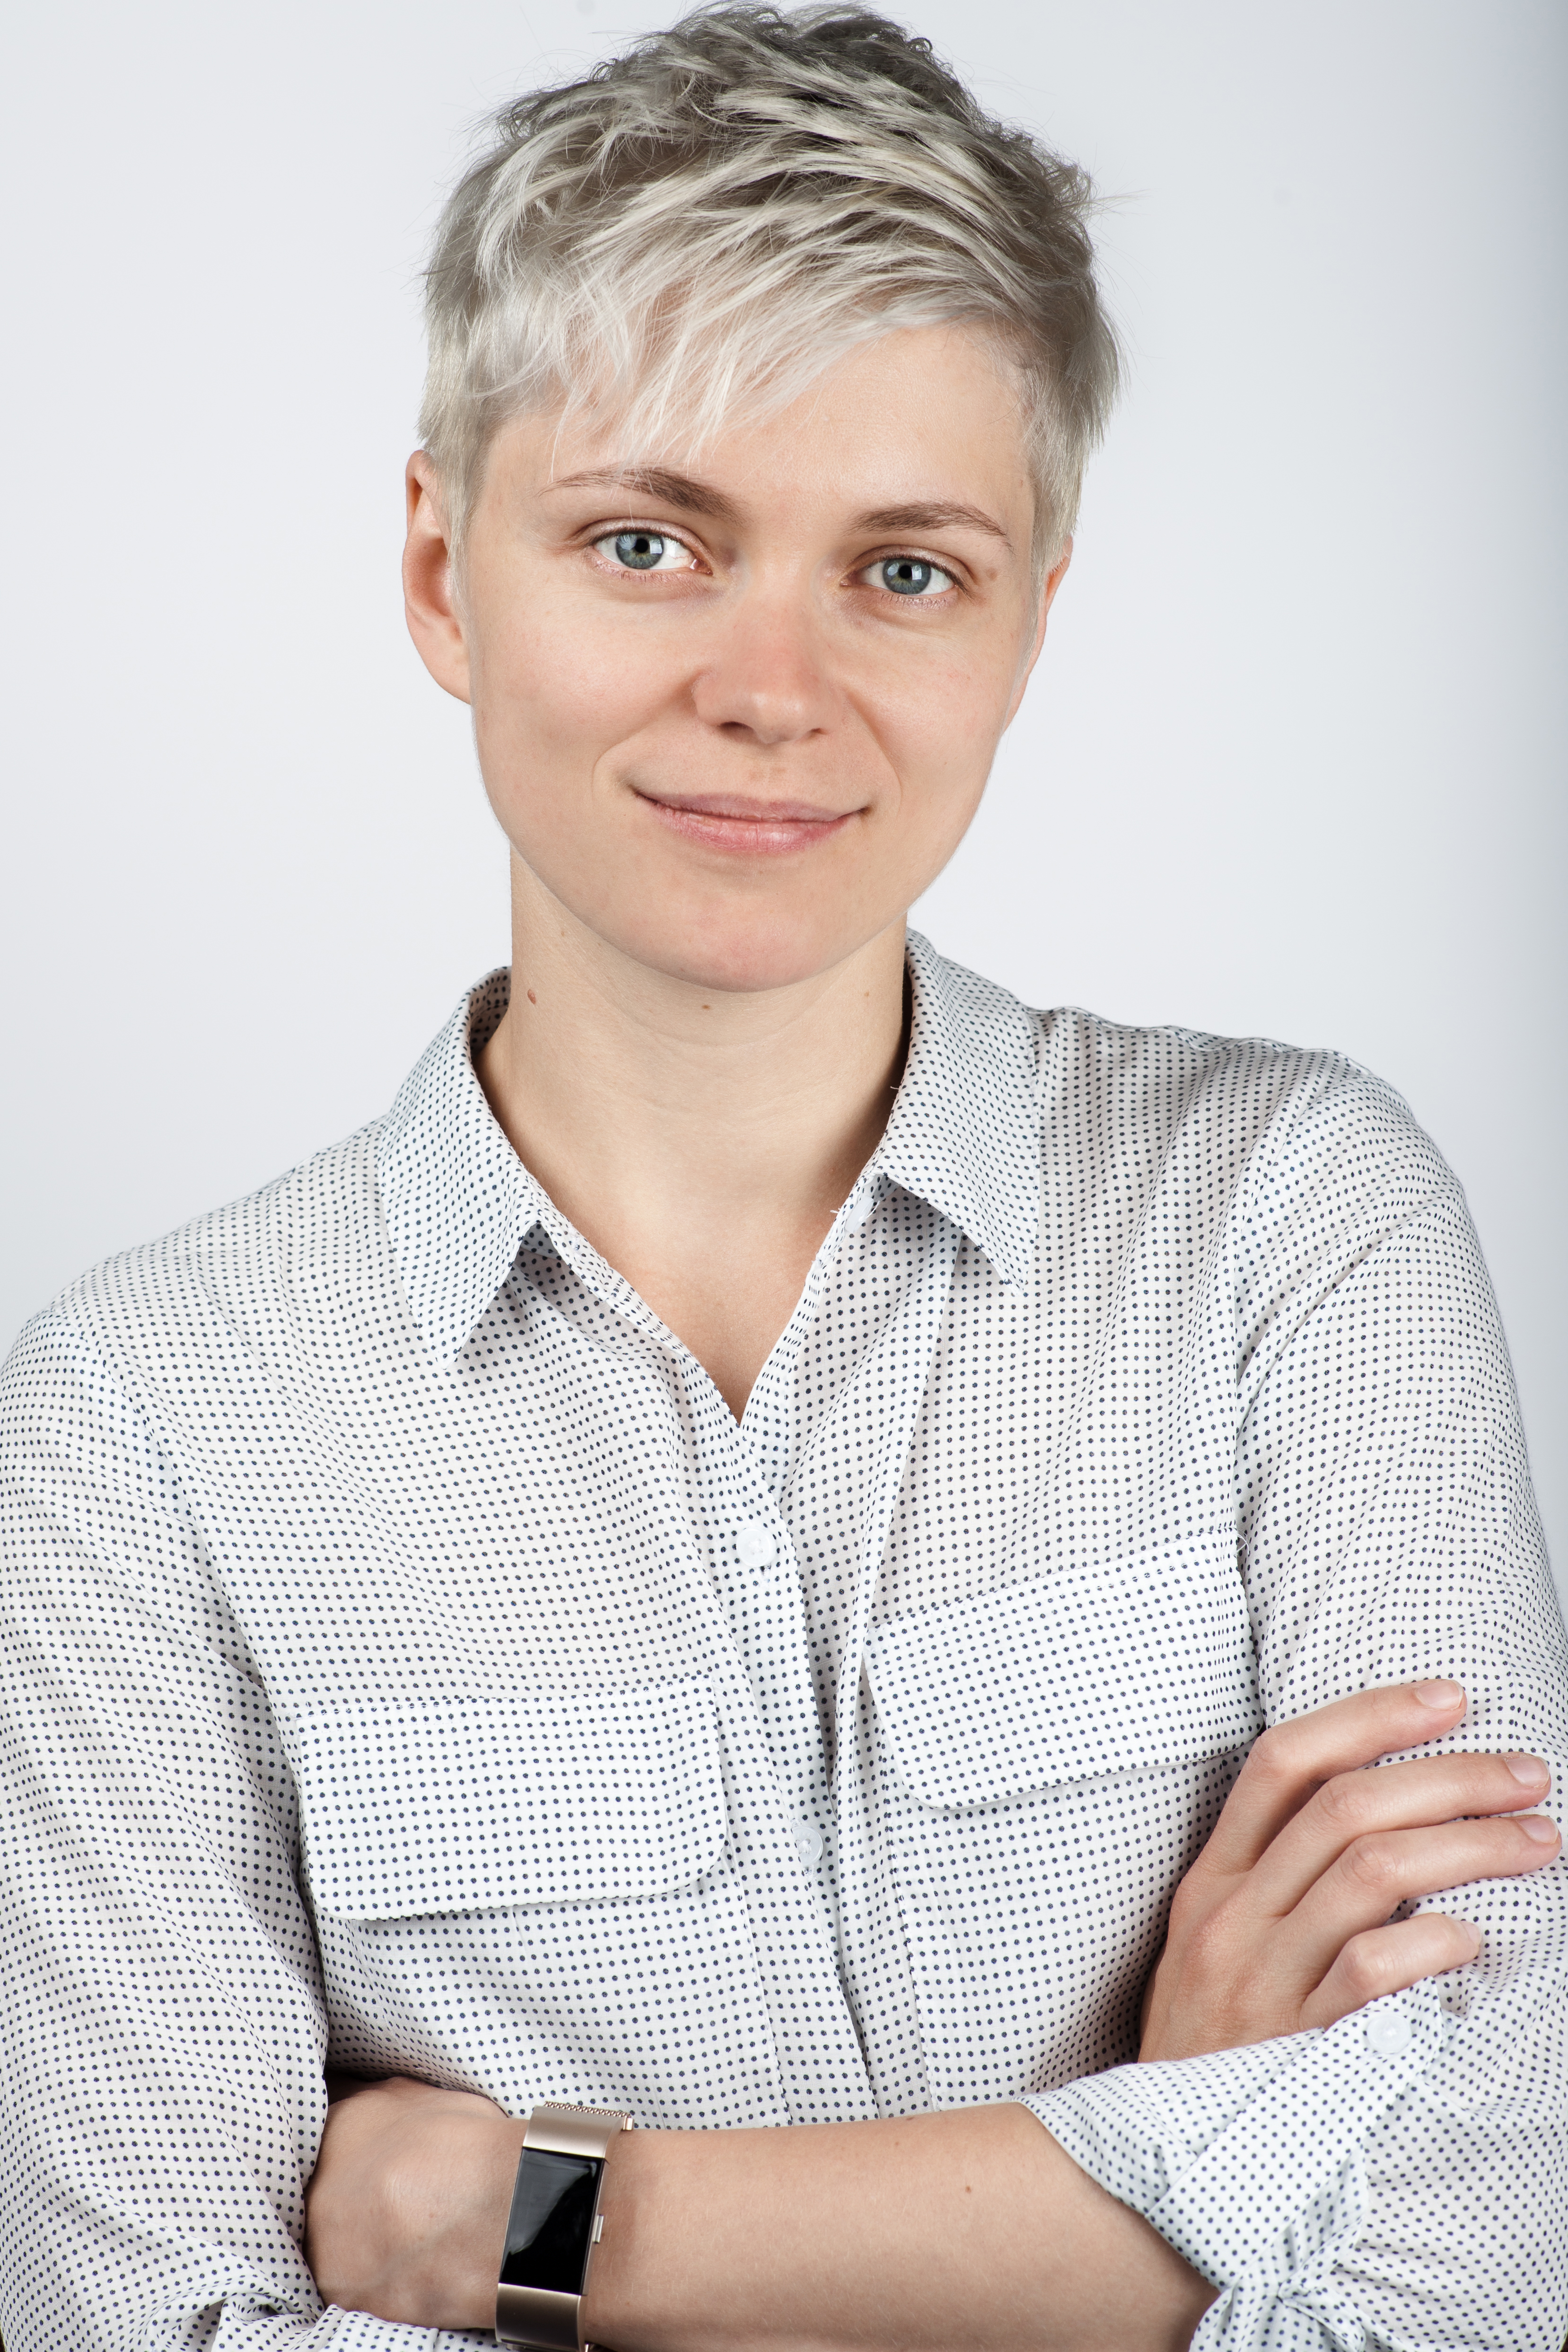
\includegraphics[width=0.67\textwidth]{nadia_polikarpova.jpg}\\
				Nadia Polikarpova
			\end{figure}


		\end{column}%
	\end{columns}

\end{frame}

% \begin{frame}
% 	\frametitle{Bidirectional synthesis}
%
% \end{frame}

\begin{frame}[fragile]
	\frametitle{Logically Qualified Data Types}
	\framesubtitle{Liquid Types \cite{rondon_liquid_2008}}

	Liquid Types is a way for automatically deriving \hl{refinement types}.

	\begin{block}{Refinement types}
		A combination of a ``regular type'' and a \textbf{refinement}.\\
		A refinement is a logic restriction on the values of the type.\\
	\end{block}

	\pause

	\begin{exampleblock}{Example}
		\vspace*{-.2\baselineskip}
		\begin{lstlisting}[escapechar=!,style=synquid]
i :: {!$\nu$!:Int | 1 !$\le$! !$\nu$! !$\wedge$! !$\nu$! !$\le$! 99}
		\end{lstlisting}
	\end{exampleblock}
	$\nu$ is the notation used to represent the value.
\end{frame}

\begin{frame}[fragile]
	\frametitle{Example: \texttt{replicate}}

	Taking a number $n$ and some object $x$ of type $\alpha$,\\
	return a list containing $n$ copies of $x$.\\~\\

	\begin{exampleblock}{Specification}
		\vspace*{-.2\baselineskip}
		\begin{lstlisting}[escapechar=!,style=synquid]
replicate :: n:Nat !$\mapsto$! x:!$\color{fibeamer@color1}{\alpha}$! !$\mapsto$! {!$\nu$!:List !$\color{fibeamer@color1}{\alpha}$! | len !$\nu$! = n}
replicate = ??
		\end{lstlisting}
	\end{exampleblock}

\end{frame}

\begin{frame}[fragile]
	\frametitle{Example: \texttt{replicate}}

	\begin{exampleblock}{Specification}
		\vspace*{-.2\baselineskip}
		\begin{lstlisting}[escapechar=!,style=synquid]
replicate :: n:Nat !$\mapsto$! x:!$\color{fibeamer@color1}{\alpha}$! !$\mapsto$! {!$\nu$!:List !$\color{fibeamer@color1}{\alpha}$! | len !$\nu$! = n}
replicate = ??
		\end{lstlisting}
	\end{exampleblock}

	\begin{exampleblock}{Auxiliary components}
		\vspace*{-.2\baselineskip}
		\begin{lstlisting}[escapechar=!,style=synquid]
zero :: {!$\nu$!:Int | !$\nu$! = 0}
inc :: x:Int !$\mapsto$! {!$\nu$!:Int | !$\nu$! = x+1}
dec :: x:Int !$\mapsto$! {!$\nu$!:Int | !$\nu$! = x-1}
leq :: x:Int !$\mapsto$! y:Int !$\mapsto$! {!$\nu$!:Bool | !$\nu$! = x!$\le$!y}
neq :: x:Int !$\mapsto$! y:Int !$\mapsto$! {!$\nu$!:Bool | !$\nu$! = x!$\neq$!y}
		\end{lstlisting}
	\end{exampleblock}

\end{frame}

\begin{frame}[allowframebreaks]
  \frametitle{References}
  \printbibliography
 \end{frame}

\end{document}
